\documentclass{article}

%----
%  Colin Tan
%  Basic setup for homework
%----
%----------------------------------------------------------------------------------------
%	PACKAGES AND OTHER DOCUMENT CONFIGURATIONS
%----------------------------------------------------------------------------------------

\usepackage{fancyhdr} % Required for custom headers
\usepackage{lastpage} % Required to determine the last page for the footer
\usepackage{extramarks} % Required for headers and footers
\usepackage{graphicx} % Required to insert images

\usepackage{listings} % listing codes

\usepackage[per-mode=symbol]{siunitx} % SI units
\usepackage{amsmath, amssymb} % Math

\usepackage{tikz} % Drawing graphs
\usepackage{pgfplots} % Drawing mathematical plots
\usepgfplotslibrary{fillbetween}
\pgfplotsset{compat=1.10} % pgf compatable version
\usepackage{float} % Flotation control

\usepackage{framed} % Framing answers
\usepackage{enumitem} % Customize enumeration style

\usepackage{multicol} % Required for columizing
\usepackage{caption} % For non-numbered captions
\usepackage{subcaption} % for caption of subfigures

\usepackage[us]{datetime} % Print date in US format

% Margins
\topmargin=-0.45in
\evensidemargin=0in
\oddsidemargin=0in
\textwidth=6.5in
\textheight=9.0in
\headsep=0.25in 

\linespread{1.1} % Line spacing

% Set up the header and footer
\pagestyle{fancy}
\lhead{\hmwkAuthorName} % Top left header
\chead{\hmwkClass\ (\hmwkClassInstructor\ \hmwkClassTime): \hmwkTitle} % Top center header
\rhead{\firstxmark} % Top right header
\lfoot{\lastxmark} % Bottom left footer
\cfoot{} % Bottom center footer
\rfoot{Page\ \thepage\ of\ \pageref{LastPage}} % Bottom right footer
\renewcommand\headrulewidth{0.4pt} % Size of the header rule
\renewcommand\footrulewidth{0.4pt} % Size of the footer rule

\setlength\parindent{0pt} % Removes all indentation from paragraphs

%----------------------------------------------------------------------------------------
%	DOCUMENT STRUCTURE COMMANDS
%----------------------------------------------------------------------------------------

% Header and footer for when a page split occurs within a problem environment
\newcommand{\enterProblemHeader}[1]{
	\nobreak\extramarks{#1}{#1 continued on next page\ldots}\nobreak
	\nobreak\extramarks{#1 (continued)}{#1 continued on next page\ldots}\nobreak
}

% Header and footer for when a page split occurs between problem environments
\newcommand{\exitProblemHeader}[1]{
	\nobreak\extramarks{#1 (continued)}{#1 continued on next page\ldots}\nobreak
	\nobreak\extramarks{#1}{}\nobreak
}

\setcounter{secnumdepth}{0} % Removes default section numbers
\newcounter{homeworkProblemCounter} % Creates a counter to keep track of the number of problems

\newcommand{\homeworkProblemName}{}
\newenvironment{homeworkProblem}[1][Problem \arabic{homeworkProblemCounter}]{ % Makes a new environment called homeworkProblem which takes 1 argument (custom name) but the default is "Problem #"
	\stepcounter{homeworkProblemCounter} % Increase counter for number of problems
	\renewcommand{\homeworkProblemName}{#1} % Assign \homeworkProblemName the name of the problem
	\section{\homeworkProblemName} % Make a section in the document with the custom problem count
	\enterProblemHeader{\homeworkProblemName} % Header and footer within the environment
}{
	\exitProblemHeader{\homeworkProblemName} % Header and footer after the environment
}

\newcommand{\problemAnswer}[1]{ % Defines the problem answer command with the content as the only argument
	\noindent\begin{oframed}
		#1
	\end{oframed}
}

\newcommand{\homeworkSectionName}{}
\newenvironment{homeworkSection}[1]{ % New environment for sections within homework problems, takes 1 argument - the name of the section
	\renewcommand{\homeworkSectionName}{#1} % Assign \homeworkSectionName to the name of the section from the environment argument
	\subsection{\homeworkSectionName} % Make a subsection with the custom name of the subsection
	\enterProblemHeader{\homeworkProblemName\ [\homeworkSectionName]} % Header and footer within the environment
}{
	\enterProblemHeader{\homeworkProblemName} % Header and footer after the environment
}

%----------------------------------------------------------------------------------------
%	TITLE PAGE
%----------------------------------------------------------------------------------------

\title{
\vspace{2in}
\textmd{\textbf{\hmwkClass:\ \hmwkTitle}}\\
\normalsize\vspace{0.1in}\small{Due\ on\ \hmwkDueDate}\\
\vspace{0.1in}\large{\textit{\hmwkClassInstructor\ \hmwkClassTime}}
\vspace{3in}
}

\author{\textbf{\hmwkAuthorName}}
\date{\today} % Insert date here if you want it to appear below your name

\usetikzlibrary{shapes.geometric, calc}
%\everymath{\displaystyle}
%----------------------------------------------------------------------------------------
%	NAME AND CLASS SECTION
%----------------------------------------------------------------------------------------

\newdate{DueDate}{18}{03}{2015} % Due date in {dd}{mm}{yyyy}
\newcommand{\hmwkTitle}{Homework\ 7} % Assignment title
\newcommand{\hmwkDueDate}{\dayofweekname{\getdateday{DueDate}}{\getdatemonth{DueDate}}{\getdateyear{DueDate}} \displaydate{DueDate}} % Due date
\newcommand{\hmwkClass}{PHYS\ 161} % Course/class
\newcommand{\hmwkClassTime}{11:00am} % Class/lecture time
\newcommand{\hmwkClassInstructor}{Professor Landee} % Teacher/lecturer
\newcommand{\hmwkAuthorName}{Zhuoming Tan} % Your name

%----------------------------------------------------------------------------------------

\begin{document}

\maketitle
\newpage
%----------------------------------------------------------------------------------------
%	TABLE OF CONTENTS
%----------------------------------------------------------------------------------------

%\setcounter{tocdepth}{1} % Uncomment this line if you don't want subsections listed in the ToC

%\newpage
%\tableofcontents
%\newpage

%----------------------------------------------------------------------------------------
%	PROBLEM 1
%----------------------------------------------------------------------------------------

% To have just one problem per page, simply put a \clearpage after each problem

\begin{homeworkProblem}
	(6.10) \textit{Rings with opposite currents}

	Two parallel rings have the same axis and are separated by a small distance $\epsilon$. They have the same radius $a$, and they carry the same current $I$ but in opposite directions. Consider the magnetic field at points on the axis of the rings. The field is zero midway between the rings, because the contributions from the rings cancel. And the field is zero very far away. So it must reach a maximum value at some point in between. Find this point. Work in the approximation where $\epsilon\ll a$.
	% Question

	\textbf{Solution}

	From the equation for field on axis
	\begin{equation}\tag{6.53}
		B_z=\frac{\mu_0Ib^2}{2(b^2+z^2)^{3/2}}
	\end{equation}
	the field for this set up on the z axis would be
	\[
		B_z=\frac{\mu_0Ia^2}{2}\left(\frac{1}{(a^2+(z-\epsilon/2)^2)^{3/2}}-\frac{1}{(a^2+(z+\epsilon/2)^2)^{3/2}}\right)
	\]
	the first order Taylor expansion is
	\[
		B_z\approx\frac{\mu_0Ia^2}{2}\frac{3z\epsilon}{\left(a^2+z^2\right)^{5/2}}
	\]
	Now let constant $k=\frac{\mu_0Ia^2}{2}$,
	\[
		\frac{B_z}{k}=\frac{3z\epsilon}{\left(a^2+z^2\right)^{5/2}}
	\]
	So take derivative,
	\[
		\frac{d}{dz}\frac{B_z}{k}=\frac{3\epsilon\left(a^2-4z^2\right)}{\left(a^2+z^2\right)^{7/2}}
	\]
	and let it equals zero. It yields that $z=a/2$. Put this result into the equation, the maximum value is:
	\[
		\frac{24\epsilon\mu_0I}{25\sqrt{5}a^2}
	\]
\end{homeworkProblem}

%----------------------------------------------------------------------------------------
%	PROBLEM 2
%----------------------------------------------------------------------------------------

\begin{homeworkProblem}
	(6.44) \textit{Line integral along the axis}

	Consider the magnetic field of a circular current ring, at points on the axis of the ring, given by Eq.~(6.53). Calculate explicitly the line integral of the field along the axis from $-\infty$ to $\infty$, to check the general formula
	\begin{equation}\tag{6.97}
		\int\mathbf{B}\cdot d\mathbf{s}=\mu_0I
	\end{equation}
	Why may we ignore the ``return'' part of the path which would be necessary to complete a closed loop?
	% Question

	\textbf{Solution}

	Let us mention the equation
	\begin{equation}\tag{6.53}
		B_z=\frac{\mu_0Ib^2}{2(b^2+z^2)^{3/2}}
	\end{equation}
	So the integral
	\[
		\int\mathbf{B}\cdot d\mathbf{s}=\int_{-\infty}^{\infty}\frac{\mu_0Ib^2}{2(b^2+z^2)^{3/2}}\,dz=\frac{\mu_0I}{2}\int_{-\infty}^{\infty}\frac{b^2}{(b^2+z^2)^{3/2}}\,dz=\left.\frac{\mu_0I}{2}\frac{z}{\sqrt{b^2+z^2}}\right|_{-\infty}^{\infty}=\mu_0I
	\]
	This integral goes from $-\infty$ to $\infty$, therefore the return part would be infinitesimally small, which could be ignored.
\end{homeworkProblem}

%----------------------------------------------------------------------------------------
%	PROBLEM 3
%----------------------------------------------------------------------------------------

\begin{homeworkProblem}
	(6.54) \textit{Force between a wire and a loop}
	
	Figure~6.47 shows a horizontal infinite straight wire with current $I_1$ pointing into the page, passing a height $z$ above a square horizontal loop with side length $l$ and current $I_2$... (problem omitted)
	\begin{figure}[H]
		\centering
		\begin{tikzpicture}
			\draw[thick] (-2,0) -- (2,0);
			\draw[thick] (-1.7,1) -- (1.7,1);
			\draw[thick] (-1.7,1) -- (-2,0);
			\draw[thick] (1.7,1) -- (2,0) node[midway, right] {$l$};
			\draw[dashed] (0,0.5) -- (0,5) node[midway, left] {$z$};
			\fill (0,5) circle[radius=0.1];
		\end{tikzpicture}
		\caption{Figure~6.47}
	\end{figure}
	% Question

	\textbf{Solution}

	From this front view
	\begin{figure}[H]
		\centering
		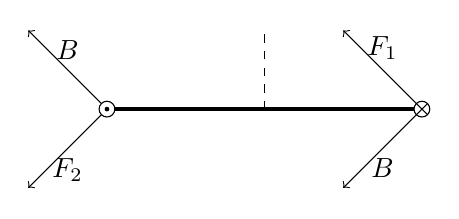
\begin{tikzpicture}
			\draw[very thick] (-2,0) -- (2,0);
			\draw[dashed] (0,0) -- (0,1);
			\draw[->] (2,0) -- (1,-1) node[midway, below] {$B$};
			\draw[->] (2,0) -- (1,1) node[midway, above] {$F_1$};
			\draw[->] (-2,0) -- (-3,1) node[midway, above] {$B$};
			\draw[->] (-2,0) -- (-3,-1) node[midway, below] {$F_2$};
			\filldraw[fill=white, draw=black] (2,0) circle[radius=0.1];
			\draw (2.0707,0.0707) -- (1.9293,-0.0707);
			\draw (1.9293,0.0707) -- (2.0707,-0.0707);
			\filldraw[fill=white, draw=black] (-2,0) circle[radius=0.1];
			\fill[black] (-2,0) circle[radius=0.03];
		\end{tikzpicture}
	\end{figure}
	the net force $F_1+F_2$ on the square is indeed to the left. Because the circular magnetic field due to $I_1$ is
	\[
		B=\frac{\mu_0I_1}{2\pi R}
	\]
	the force $F_1$ on the right side is
	\[
		F_1=I_2lB=\frac{\mu_0I_1I_2l}{2\pi R}
	\]
	with the angle $\theta$ to the $x$ direction, where $\cos\theta=\frac{l/2}{R}$. So its $x$ component is
	\[
		F_{1x}=\frac{\mu_0I_1I_2l}{2\pi R}\frac{l/2}{R}=\frac{\mu_0I_1I_2l^2}{4\pi R^2}
	\]
	and $F_{2x}$ could be shown as the same. Therefore the net force equals
	\[
		F=F_{1x}+F_{2x}=\frac{\mu_0I_1I_2l^2}{2\pi R^2}
	\]
\end{homeworkProblem}

%----------------------------------------------------------------------------------------
%	PROBLEM 4
%----------------------------------------------------------------------------------------

\begin{homeworkProblem}
	The square coil.

	Consider a square coil with the length of each side is $a$. A current $I$ is passed through the ring. Calculate the magnetic field on the vertical axis that passes through the center of the square. Compare this field to that of a circular loop with the same current and a diameter $a$.
	% Question

	\textbf{Solution}

	\begin{figure}[H]
		\centering
		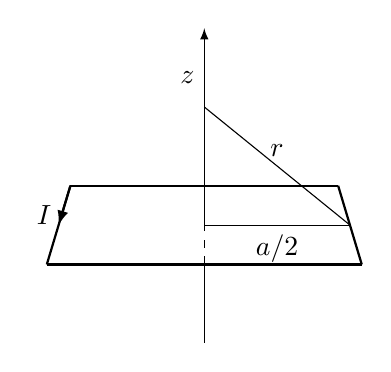
\begin{tikzpicture}
			\draw[thick] (-2,0) -- (2,0);
			\draw[thick] (-1.7,1) -- (1.7,1);
			\draw[thick] (-1.7,1) -- (-2,0);
			\draw[-latex, thick] (-1.7,1) -- (-1.85,0.5) node[near end, left] {$I$};
			\draw[thick] (1.7,1) -- (2,0);
			\draw[-latex] (0,0.5) -- (0,3) node[near end, left] {$z$};
			\draw (0,0.5) -- (1.85,0.5) node[midway, below] {$a/2$};
			\draw (0,2) -- (1.85,0.5) node[midway, above] {$r$};
			\draw[dashed] (0,0) -- (0,0.5);
			\draw(0,0) -- (0,-1);
		\end{tikzpicture}
	\end{figure}

	The Biot-Savart law says that
	\[
		\mathbf{B}(\mathbf{r})=\frac{\mu_0I}{4\pi}\int\frac{d\mathbf{l}\times\mathbf{r}}{|\mathbf{r}|^3}
	\]
	where $\mathbf{r}$ is the displacement vector. Now consider the right edge. $\mathbf{r}=(0-a/2)\hat{x}+(0-y)\hat{y}+(z-0)\hat{z}$. $d\mathbf{l}=dy\hat{y}$. Therefore $d\mathbf{l}\times\mathbf{r}=\left(z\hat{x}+\frac{a}{2}\hat{z}\right)dy$. So the integral
	\[
		\mathbf{B}_1=\frac{\mu_0I}{4\pi}\left(z\hat{x}+\frac{a}{2}\hat{z}\right)\int_{-a/2}^{a/2}\frac{dy}{(\frac{a^2}{4}+y^2+z^2)^{3/2}}=\frac{\mu_0I}{4\pi}\left(z\hat{x}+\frac{a}{2}\hat{z}\right)\frac{4a}{\sqrt{\frac{a^2}{2}+z^2}\left(a^2+4z^2\right)}
	\]
	By symmetry of the configuration, the segment on left would contribute the same $\hat{z}$ component but opposite $\hat{x}$ component. By the same reason, the two top and bottom segments will do the same. Therefore the total field would be
	\[
		\mathbf{B}=4\times\frac{\mu_0I}{4\pi}\frac{a}{2}\hat{z}\frac{4a}{\sqrt{\frac{a^2}{2}+z^2}\left(a^2+4z^2\right)}=\frac{2a^2\mu_0I}{\pi\sqrt{\frac{a^2}{2}+z^2}\left(a^2+4z^2\right)}\hat{z}
	\]
	Comparing to the field on axis for a circular loop which is
	\[
		\mathbf{B}'=\frac{a^2\mu_0I}{\left(a^2+z^2\right)^{3/2}}\hat{z}
	\]
	Their ratio
	\[
		\lim_{z\rightarrow\infty}\frac{\mathbf{B}}{\mathbf{B}'}=\lim_{z\rightarrow\infty}\frac{2\left(a^2+z^2\right)^{3/2}}{\pi\sqrt{\frac{a^2}{2}+z^2}\left(a^2+4z^2\right)}=\frac{1}{2\pi}
	\]
\end{homeworkProblem}

%----------------------------------------------------------------------------------------
%	PROBLEM 5
%----------------------------------------------------------------------------------------

\begin{homeworkProblem}
	(III-8) In the text (pages 82-86) we obtained... (problem omitted)
	% Question

	\textbf{Solution}

	% r
	For the $r$ coordinate, mark the side on the left going down as 1, and so on.
	\[
		\oint_{C_1}\mathbf{F}\cdot\hat{\mathbf{t}}\,ds\simeq-F_z\left(r,\theta-\frac{\Delta\theta}{2},z\right)\Delta z
	\]
	\[
		\oint_{C_3}\mathbf{F}\cdot\hat{\mathbf{t}}\,ds\simeq F_z\left(r,\theta+\frac{\Delta\theta}{2},z\right)\Delta z
	\]
	And the area enclosed is $r\Delta\theta\Delta z$. So
	\[
		\frac{1}{\Delta S}\int_{C_1+C_3}\mathbf{F}\cdot\hat{\mathbf{t}}\,ds=\frac{1}{r\Delta\theta}\left[F_z\left(r,\theta+\frac{\Delta\theta}{2},z\right)-F_z\left(r,\theta-\frac{\Delta\theta}{2},z\right)\right]
	\]
	Take the limit to $\Delta\theta\rightarrow0$, this becomes
	\[
		\frac{1}{r}\frac{\partial F_z}{\partial\theta}
	\]
	Then
	\[
		\oint_{C_2}\mathbf{F}\cdot\hat{\mathbf{t}}\,ds\simeq F_\theta\left(r,\theta,z-\frac{\Delta z}{2}\right)r\Delta\theta
	\]
	\[
		\oint_{C_4}\mathbf{F}\cdot\hat{\mathbf{t}}\,ds\simeq-F_\theta\left(r,\theta,z+\frac{\Delta z}{2}\right)r\Delta\theta
	\]
	so
	\[
		\frac{1}{\Delta S}\int_{C_2+C_4}\mathbf{F}\cdot\hat{\mathbf{t}}\,ds=-\frac{1}{\Delta z}\left[F_\theta\left(r,\theta,z+\frac{\Delta z}{2}\right)-F_\theta\left(r,\theta,z-\frac{\Delta z}{2}\right)\right]
	\]
	Take the limit to $\Delta z\rightarrow0$, this becomes
	\[
		-\frac{\partial F_\theta}{\partial z}
	\]
	Therefore we could conclude
	\[
		(\nabla\times\mathbf{F})_r=\frac{1}{r}\frac{\partial F_z}{\partial\theta}-\frac{\partial F_\theta}{\partial z}
	\]

	% \theta
	Similarly for the $\theta$ coordinate, mark the side closest to $z$ axis going up as 1, and so on.
	\[
		\oint_{C_1}\mathbf{F}\cdot\hat{\mathbf{t}}\,ds\simeq F_z\left(r-\frac{\Delta r}{2},\theta,z\right)\Delta z
	\]
	\[
		\oint_{C_3}\mathbf{F}\cdot\hat{\mathbf{t}}\,ds\simeq-F_z\left(r+\frac{\Delta r}{2},\theta,z\right)\Delta z
	\]
	And the area enclosed is $\Delta r\Delta z$. So
	\[
		\frac{1}{\Delta S}\int_{C_1+C_3}\mathbf{F}\cdot\hat{\mathbf{t}}\,ds=-\frac{1}{\Delta r}\left[F_z\left(r+\frac{\Delta r}{2},\theta,z\right)-F_z\left(r-\frac{\Delta r}{2},\theta,z\right)\right]
	\]
	Take the limit to $\Delta r\rightarrow0$, this becomes
	\[
		-\frac{\partial F_z}{\partial r}
	\]
	Then
	\[
		\oint_{C_2}\mathbf{F}\cdot\hat{\mathbf{t}}\,ds\simeq F_r\left(r,\theta,z+\frac{\Delta z}{2}\right)\Delta r
	\]
	\[
		\oint_{C_4}\mathbf{F}\cdot\hat{\mathbf{t}}\,ds\simeq-F_r\left(r,\theta,z-\frac{\Delta z}{2}\right)\Delta r
	\]
	so
	\[
		\frac{1}{\Delta S}\int_{C_2+C_4}\mathbf{F}\cdot\hat{\mathbf{t}}\,ds=\frac{1}{\Delta z}\left[F_r\left(r,\theta,z+\frac{\Delta z}{2}\right)-F_r\left(r,\theta,z+\frac{\Delta z}{2}\right)\right]
	\]
	Take the limit to $\Delta z\rightarrow0$, this becomes
	\[
		\frac{\partial F_r}{\partial z}
	\]
	Therefore we could conclude
	\[
		(\nabla\times\mathbf{F})_\theta=\frac{\partial F_r}{\partial z}-\frac{\partial F_z}{\partial r}
	\]
\end{homeworkProblem}

%----------------------------------------------------------------------------------------
%	PROBLEM 6
%----------------------------------------------------------------------------------------

\begin{homeworkProblem}
	(III-9) Following the procedure... (problem omitted)
	% Question

	\textbf{Solution}

	% r
	For the $r$ coordinate,
	\[
		\oint_{C_1}\mathbf{F}\cdot\hat{\mathbf{t}}\,ds\simeq F_\phi\left(r,\phi,\theta-\frac{\Delta\theta}{2}\right)r\Delta\phi
	\]
	\[
		\oint_{C_3}\mathbf{F}\cdot\hat{\mathbf{t}}\,ds\simeq-F_\phi\left(r,\phi,\theta+\frac{\Delta\theta}{2}\right)r\Delta\phi
	\]
	And the area enclosed is $r^2\Delta\theta\Delta\phi\sin\phi$. So
	\[
		\frac{1}{\Delta S}\int_{C_1+C_3}\mathbf{F}\cdot\hat{\mathbf{t}}\,ds=-\frac{1}{r\Delta\theta\sin\phi}\left[F_\phi\left(r,\phi,\theta+\frac{\Delta\theta}{2}\right)-F_\phi\left(r,\phi,\theta-\frac{\Delta\theta}{2}\right)\right]
	\]
	Take the limit to $\Delta\theta\rightarrow0$, this becomes
	\[
		-\frac{1}{r\sin\phi}\frac{\partial F_\phi}{\partial\theta}
	\]
	Then
	\[
		\oint_{C_2}\mathbf{F}\cdot\hat{\mathbf{t}}\,ds\simeq-F_\theta\left(r,\phi-\frac{\Delta\phi}{2},\theta\right)r\sin\left(\phi-\frac{\Delta\phi}{2}\right)\Delta\pi
	\]
	\[
		\oint_{C_4}\mathbf{F}\cdot\hat{\mathbf{t}}\,ds\simeq F_\theta\left(r,\phi+\frac{\Delta\phi}{2},\theta\right)r\sin\left(\phi+\frac{\Delta\phi}{2}\right)\Delta\phi
	\]
	so
	\[
		\frac{1}{\Delta S}\int_{C_2+C_4}\mathbf{F}\cdot\hat{\mathbf{t}}\,ds=\frac{1}{r\Delta\theta\sin\phi}\left[F_\theta\left(r,\phi+\frac{\Delta\phi}{2},\theta\right)\sin\left(\phi+\frac{\Delta\phi}{2}\right)-F_\theta\left(r,\phi-\frac{\Delta\phi}{2},\theta\right)\sin\left(\phi-\frac{\Delta\phi}{2}\right)\right]
	\]
	Take the limit to $\Delta\theta\rightarrow0$, this becomes
	\[
		\frac{1}{r\sin\phi}\frac{\partial}{\partial\phi}(\sin\phi F_\theta)
	\]
	Therefore we could conclude
	\[
		(\nabla\times\mathbf{F})_r=\frac{1}{r\sin\phi}\frac{\partial}{\partial\phi}(\sin\phi F_\theta)-\frac{1}{r\sin\phi}\frac{\partial F_\phi}{\partial\theta}
	\]

	% \phi
	For the $\phi$ coordinate, enclosed area is $r\Delta r\Delta\theta\sin\phi$
	\[
		\oint_{C_1}\mathbf{F}\cdot\hat{\mathbf{t}}\,ds\simeq-F_\theta\left(r+\frac{\Delta r}{2},\phi,\theta\right)\left(r+\frac{\Delta r}{2}\right)\Delta\theta\sin\phi
	\]
	\[
		\oint_{C_2}\mathbf{F}\cdot\hat{\mathbf{t}}\,ds\simeq-F_r\left(r,\phi,\theta-\frac{\Delta\theta}{2}\right)\Delta r
	\]
	\[
		\oint_{C_3}\mathbf{F}\cdot\hat{\mathbf{t}}\,ds\simeq F_\theta\left(r-\frac{\Delta r}{2},\phi,\theta\right)\left(r-\frac{\Delta r}{2}\right)\Delta\theta\sin\phi
	\]
	\[
		\oint_{C_4}\mathbf{F}\cdot\hat{\mathbf{t}}\,ds\simeq F_r\left(r,\phi,\theta+\frac{\Delta\theta}{2}\right)\Delta r
	\]
	so
	\[
		\frac{1}{\Delta S}\int_{C_1+C_3}\mathbf{F}\cdot\hat{\mathbf{t}}\,ds=-\frac{1}{r\Delta r}\left[F_\theta\left(r+\frac{\Delta r}{2},\phi,\theta\right)\left(r+\frac{\Delta r}{2}\right)-F_\theta\left(r-\frac{\Delta r}{2},\phi,\theta\right)\left(r-\frac{\Delta r}{2}\right)\right]
	\]
	\[
		\frac{1}{\Delta S}\int_{C_2+C_4}\mathbf{F}\cdot\hat{\mathbf{t}}\,ds=\frac{1}{r\Delta\theta\sin\phi}\left[F_r\left(r,\phi,\theta+\frac{\Delta\theta}{2}\right)-F_r\left(r,\phi,\theta-\frac{\Delta\theta}{2}\right)\right]
	\]
	Take the limits, we could conclude
	\[
		(\nabla\times\mathbf{F})_\phi=\frac{1}{r\sin\phi}\frac{\partial F_r}{\partial\theta}-\frac{1}{r}\frac{\partial}{\partial\theta}(rF_\theta)
	\]

	% \theta
	For the $\theta$ coordinate, enclosed area is $r\Delta r\Delta\phi$
	\[
		\oint_{C_1}\mathbf{F}\cdot\hat{\mathbf{t}}\,ds\simeq F_\phi\left(r+\frac{\Delta r}{2},\phi,\theta\right)\left(r+\frac{\Delta r}{2}\right)\Delta\phi
	\]
	\[
		\oint_{C_2}\mathbf{F}\cdot\hat{\mathbf{t}}\,ds\simeq-F_r\left(r,\phi-\frac{\Delta\phi}{2},\theta\right)\Delta r
	\]
	\[
		\oint_{C_3}\mathbf{F}\cdot\hat{\mathbf{t}}\,ds\simeq-F_\phi\left(r-\frac{\Delta r}{2},\phi,\theta\right)\left(r-\frac{\Delta r}{2}\right)\Delta\phi
	\]
	\[
		\oint_{C_4}\mathbf{F}\cdot\hat{\mathbf{t}}\,ds\simeq F_r\left(r,\phi+\frac{\Delta\phi}{2},\theta\right)\Delta r
	\]
	so
	\[
		\frac{1}{\Delta S}\int_{C_1+C_3}\mathbf{F}\cdot\hat{\mathbf{t}}\,ds=\frac{1}{r\Delta r}\left[F_\phi\left(r+\frac{\Delta r}{2},\phi,\theta\right)\left(r+\frac{\Delta r}{2}\right)-F_\phi\left(r-\frac{\Delta r}{2},\phi,\theta\right)\left(r-\frac{\Delta r}{2}\right)\right]
	\]
	\[
		\frac{1}{\Delta S}\int_{C_2+C_4}\mathbf{F}\cdot\hat{\mathbf{t}}\,ds=-\frac{1}{r\Delta\phi}\left[F_r\left(r,\phi+\frac{\Delta\phi}{2},\theta\right)-F_r\left(r,\phi-\frac{\Delta\phi}{2},\theta\right)\right]
	\]
	Take the limits, we could conclude
	\[
		(\nabla\times\mathbf{F})_\theta=\frac{1}{r}\frac{\partial}{\partial r}(rF_\phi)-\frac{1}{r}\frac{\partial F_r}{\partial\phi}
	\]
\end{homeworkProblem}

%----------------------------------------------------------------------------------------
%	PROBLEM 7
%----------------------------------------------------------------------------------------

\begin{homeworkProblem}
	(III-15) Verify Stokes' theorem
	\[
		\oint_C\mathbf{F}\cdot\hat{\mathbf{t}}\,ds=\iint_S\hat{\mathbf{n}}\cdot\nabla\times\mathbf{F}\,dS
	\]
	in each of the following cases... (problem omitted)
	% Question

	\textbf{Solution}
	\begin{enumerate}[label=(\alph*)]
		\begin{item}
		 	\[
			 	\nabla\times\mathbf{F}=\begin{vmatrix}
			 		i & j & k \\
			 		\frac{\partial}{\partial x} & \frac{\partial}{\partial y} & \frac{\partial}{\partial z} \\
			 		F_x & F_y & F_z \\
			 	\end{vmatrix}=2z\hat{\mathbf{j}}
		 	\]
		 	Therefore, at $y=0$
		 	\[
			 	\iint_S\hat{\mathbf{n}}\cdot\nabla\times\mathbf{F}\,dS=\int_0^1\int_0^1\hat{\mathbf{j}}\cdot2z\hat{\mathbf{j}}\,dx\,dz=\int_0^1\int_0^1 2z\,dx\,dz=1
		 	\]
		 	And
		 	\begin{align*}
				\oint_C\mathbf{F}\cdot\hat{\mathbf{t}}\,ds&=\int_0^1\mathbf{F}(x,y,z=1)\cdot\hat{\mathbf{i}}\,dx-\int_0^1\mathbf{F}(x=1,y,z)\cdot\hat{\mathbf{k}}\,dz \\
				&-\int_0^1\mathbf{F}(x,y,z=0)\cdot\hat{\mathbf{i}}\,dx+\int_0^1\mathbf{F}(x=0,y,z)\cdot\hat{\mathbf{k}}\,dz \\
				&=1-0-0+0=1
			\end{align*}
			As shown, Stokes' theorem holds in this case.
		\end{item}
		\begin{item}
			\[
				\oint_C\mathbf{F}\cdot\hat{\mathbf{t}}\,ds=\int_{C_1}\mathbf{F}\cdot\hat{\mathbf{t}}\,ds+\int_{C_2}\mathbf{F}\cdot\hat{\mathbf{t}}\,ds+\int_{C_3}\mathbf{F}\cdot\hat{\mathbf{t}}\,ds
			\]
			Parametrize the paths.

			For $C_1$, $r=1$, $\theta=\pi/2$, so $\hat{\mathbf{r}}(\phi)=(\cos\phi,\sin\phi,0)$, where $0\leq\phi\leq\pi/2$. And $\mathbf{f}(\phi)=(\sin\phi,0,\cos\phi)$. The integral becomes
			\[
				\int_{C_1}\mathbf{F}\cdot\hat{\mathbf{t}}\,ds=\int_0^{\pi/2}\mathbf{f}\cdot\hat{\mathbf{r}}'\,d\phi=\int_0^{\pi/2}-\sin^2\phi\,d\phi=-\frac{\pi}{4}
			\]

			For $C_2$, $r=1$, $\phi=\pi/2$, so $\hat{\mathbf{r}}(\theta)=(0,\cos\theta,\sin\theta)$, where $0\leq\theta\leq\pi/2$. And $\mathbf{f}(\theta)=(\cos\theta,\sin\theta,0)$. The integral becomes
			\[
				\int_{C_2}\mathbf{F}\cdot\hat{\mathbf{t}}\,ds=\int_0^{\pi/2}\mathbf{f}\cdot\hat{\mathbf{r}}'\,d\theta=\int_0^{\pi/2}-\sin^2\theta\,d\theta=-\frac{\pi}{4}
			\]

			For $C_3$, $r=1$, $\phi=0$, so $\hat{\mathbf{r}}(\theta)=(\cos\theta,0,\sin\theta)$, where $0\leq\theta\leq\pi/2$. And $\mathbf{f}(\theta)=(0,\sin\theta,\cos\theta)$. The integral becomes
			\[
				\int_{C_3}\mathbf{F}\cdot\hat{\mathbf{t}}\,ds=\int_0^{\pi/2}\mathbf{f}\cdot\hat{\mathbf{r}}'\,d\theta=\int_0^{\pi/2}-\cos^2\theta\,d\theta=-\frac{\pi}{4}
			\]
			So adding these up,
			\[
				\oint_C\mathbf{F}\cdot\hat{\mathbf{t}}\,ds=-\frac{3\pi}{4}
			\]
			$\nabla\times\mathbf{F}=(-1,-1,-1)$. Change into spherical coordinates, $\nabla\times\mathbf{F}=\left(\sqrt{3},\pi-\tan^{-1}\left(\sqrt{2}\right),-\frac{3\pi}{4}\right)$. The normal vector $\hat{\mathbf{n}}=x\hat{\mathbf{i}}+y\hat{\mathbf{j}}+z\hat{\mathbf{k}}$, therefore $\hat{\mathbf{n}}\cdot\nabla\times\mathbf{F}=-x-y-z$. So when $r=1$
			\begin{align*}
				\iint_S\hat{\mathbf{n}}\cdot\nabla\times\mathbf{F}\,dS&=\iint_S(-x-y-z)\,dS \\
				&=-\int_0^{\pi/2}\int_0^{\pi/2}(x+y+z)r^2\sin\theta\,d\phi\,d\theta \\
				&=-\int_0^{\pi/2}\int_0^{\pi/2}(\sin\phi\sin\theta+\cos\phi\sin\theta+\cos\theta)\sin\theta\,d\phi\,d\theta \\
				&=-\frac{3\pi}{4}
			\end{align*}
			Stokes' theorem holds in this case.
		\end{item}
		\begin{item}
			$\nabla\times\mathbf{F}=(0,0,-2)$, so in cylindrical coordinates
			\begin{align*}
				\iint_S\hat{\mathbf{n}}\cdot\nabla\times\mathbf{F}\,dS&=\iint_S\hat{\mathbf{n}}\cdot(0,0,-2)\,dS \\
				&=\iint_{S_1}\hat{\mathbf{\rho}}\cdot\nabla\times\mathbf{F}\,dS+\iint_{S_2}\hat{\mathbf{z}}\cdot\nabla\times\mathbf{F}\,dS \\
				&=0+\int_0^R\int_0^{2\pi}-2\rho\,d\phi\,d\rho \\
				&=-2\pi R^2
			\end{align*}
			And then for the line integral, parametrize the path $\hat{\mathbf{r}}(\phi)=(R\cos\phi,R\sin\phi,0)$. And $\mathbf{f}=(R\sin\phi,-R\cos\phi,0)$. So
			\[
				\int_C\mathbf{F}\cdot\hat{\mathbf{t}}\,ds=\int_0^{2\pi}\mathbf{f}\cdot\hat{\mathbf{r}}'\,d\phi=\int_0^{2\pi}-R^2\,d\phi=-2\pi R^2
			\]
			Verified.
		\end{item}
	\end{enumerate}
\end{homeworkProblem}

%----------------------------------------------------------------------------------------
%	PROBLEM 8
%----------------------------------------------------------------------------------------

\begin{homeworkProblem}
	(III-16) (a) Consider a vector function with the property $\nabla\times\mathbf{F}=0$... (problem omitted)
	% Question

	\textbf{Solution}

	\begin{enumerate}[label=(\alph*)]
		\begin{item}
			Use Stokes' theorem. Because
			\[
				\oint_C\mathbf{F}\cdot\hat{\mathbf{t}}\,ds=\iint_S\hat{\mathbf{n}}\cdot\nabla\times\mathbf{F}\,dS=0
			\]
			on this dount shape, the upper and lower halves could be seen as having circulation of opposite directions, while $C_1$ or $C_2$ belongs to one of them.
			\[
				\oint_{C_1}\mathbf{F}\cdot\hat{\mathbf{t}}\,ds-\oint_{C_2}\mathbf{F}\cdot\hat{\mathbf{t}}\,ds=0
			\]
			So
			\[
				\oint_{C_1}\mathbf{F}\cdot\hat{\mathbf{t}}\,ds=\oint_{C_2}\mathbf{F}\cdot\hat{\mathbf{t}}\,ds
			\]
		\end{item}
		\begin{item}
			When assuming $r>0$, the curl
			\[
			\nabla\times\mathbf{B}=\nabla\times\left(0,\frac{\mu_0I}{2\pi r},0\right)=\left(0,0,\frac{\mu_0I}{2\pi r^2}-\frac{\mu_0I}{2\pi r^2}\right)=(0,0,0)
			\]
			When $r=0$, the calculation becomes indeterminate.
		\end{item}
		\begin{item}
			Let
			\[
				a=\oint_C\mathbf{B}\cdot\,d\mathbf{l}
			\]
			a small element of this is
			\[
				da=\mathbf{B}\cdot\,d\mathbf{r}=B\cos\theta\,dr
			\]
			When considering a cicular loop centered at $z$ axis, $\theta=0$,
			\[
				B\cos\theta\,dr=B\,dr=\frac{\mu_0I}{2\pi r}\,dr
			\]
			So
			\[
				\oint_C\mathbf{B}\cdot\,d\mathbf{l}=a=2\pi r\frac{\mu_0I}{2\pi r}=\mu_0I
			\]
			which is the Amp\`{e}re's circuital law.
		\end{item}
	\end{enumerate}
\end{homeworkProblem}

%----------------------------------------------------------------------------------------
%	PROBLEM 9
%----------------------------------------------------------------------------------------

\begin{homeworkProblem}
	(III-19) Determine the value of the line integral $\int_C\mathbf{F}\cdot\hat{\mathbf{t}},ds$ where
	\[
		\mathbf{F}=(e^{-y}-ze^{-x})\hat{\mathbf{i}}+(e^{-z}-xe^{-y})\hat{\mathbf{j}}+(e^{-x}-ye^{-z})\hat{\mathbf{k}}
	\]
	and $C$ is the path... (problem omitted)
	% Question

	\textbf{Solution}

	Firstly, calculated $\nabla\times\mathbf{F}=0$. As shown in problem 8, for a field of zero curl, two closed curves enclosing one capping surface would have the same circulation. So the path $C$ could be converted to $(0,0,0)$, $(1,0,0)$, $(1,1,0)$, and $(1,1,1)$, and still gives the same result. Therefore at $y=z=0$
	\[
		\int_0^1\left(e^{-y}-ze^{-x}\right)\,dx=1
	\]
	At $x=1$, $z=0$
	\[
		\int_0^1\left(e^{-z}-xe^{-y}\right)\,dy=\frac{1}{e}
	\]
	At $x=y=1$,
	\[
		\int_0^1\left(e^{-x}-ye^{-z}\right)\,dz=-1+\frac{2}{e}
	\]
	So the line integral is the sum of these three results, $3/e$.
\end{homeworkProblem}

%----------------------------------------------------------------------------------------
%	PROBLEM 10
%----------------------------------------------------------------------------------------

\begin{homeworkProblem}
	(III-22) (a) Apply the divergence theorem to the function
	\[
		\mathbf{G}(x,y)=\mathbf{i}G_x(x,y)+\mathbf{j}G_y(x,y)
	\]
	... (problem omitted)
	% Question

	\textbf{Solution}

	\begin{enumerate}[label=(\alph*)]
		\begin{item}
			There is no $z$ component, so
			\[
				\nabla\cdot\mathbf{G}=\frac{\partial G_x}{\partial x}+\frac{\partial G_y}{\partial y}
			\]
			Therefore
			\[
				\iiint_V\nabla\cdot\mathbf{G}\,dV=\iiint_V\left(\frac{\partial G_x}{\partial x}+\frac{\partial G_y}{\partial y}\right)\,dV=h\iint_R\left(\frac{\partial G_x}{\partial x}+\frac{\partial G_y}{\partial y}\right)\,dx\,dy
			\]
			On the other hand, the top and bottom has no contribution to the surface integral. The surface integral does not change through the $h$, so
			\begin{align*}
				\iint_S\mathbf{G}\cdot\hat{\mathbf{n}}\,dS&=h\oint_C\mathbf{G}\cdot\hat{\mathbf{n}}\,dx\,dy \\
				&=h\oint_C\left(\frac{\partial G}{\partial x}-\frac{\partial G}{\partial y}\right)\,dx\,dy \\
				&=h\oint_C\left(\frac{G_x}{dx}-\frac{G_y}{dy}\right)\,dx\,dy \\
				&=h\oint_C\left(G_x\,dy-G_y\,dx\right)
			\end{align*}
			So
			\[
				\iint_R\left(\frac{\partial G_x}{\partial x}+\frac{\partial G_y}{\partial y}\right)\,dx\,dy=\oint_C\left(G_x\,dy-G_y\,dx\right)
			\]
		\end{item}
		\begin{item}
			\[
				\nabla\times\mathbf{F}=\frac{\partial F_y}{\partial x}-\frac{\partial F_x}{\partial y}
			\]
			So
			\[
				\iint_R\nabla\times\mathbf{F}\cdot d\mathbf{S}=\iint_R\left(\frac{\partial F_y}{\partial x}-\frac{\partial F_x}{\partial y}\right)\,dx\,dy
			\]
			And
			\[
				\oint_C\mathbf{F}\cdot d\mathbf{r}=\oint_C(F_x\,dx+F_y\,dy)
			\]
			So
			\[
				\oint_C(F_x\,dx+F_y\,dy)=\iint_R\left(\frac{\partial F_y}{\partial x}-\frac{\partial F_x}{\partial y}\right)\,dx\,dy
			\]
		\end{item}
		\begin{item}
			With the result from the two problems above, just let $G_x=F_y$, and $G_y=-F_x$.
		\end{item}
	\end{enumerate}
\end{homeworkProblem}
%----------------------------------------------------------------------------------------

\end{document}
